\documentclass[10pt,english,aspectratio=169]{beamer}

\usepackage{ae,aecompl}
\usepackage[T1]{fontenc}
\usepackage{textcomp}
\usepackage[utf8]{inputenc}
\usepackage{babel}

\setcounter{secnumdepth}{3}
\setcounter{tocdepth}{3}

\usepackage{amsmath, amssymb, graphicx}
\usepackage{booktabs, multirow}
\usepackage{tikz}
\usetikzlibrary{positioning,arrows.meta,shapes,calc}
\usepackage{listings}
\usepackage{xcolor}
\usepackage{tcolorbox}

\lstset{
  basicstyle=\ttfamily\small,
  keywordstyle=\color{blue!80!black}\bfseries,
  commentstyle=\color{green!50!black}\itshape,
  stringstyle=\color{orange!80!black},
  backgroundcolor=\color{gray!8},
  frame=single,
  rulecolor=\color{gray!40},
  breaklines=true,
  showstringspaces=false,
  numbers=none,
}

\lstdefinestyle{pythonstyle}{
    language=Python,
    basicstyle=\ttfamily\footnotesize,
    keywordstyle=\color{blue!80!black}\bfseries,
    commentstyle=\color{green!50!black}\itshape,
    stringstyle=\color{orange!80!black},
    frame=single,
    rulecolor=\color{gray!40},
    backgroundcolor=\color{gray!8},
    breaklines=true,
    showstringspaces=false,
    numbers=left,
    numbersep=5pt,
    numberstyle=\tiny\color{gray}
}

\ifx\hypersetup\undefined
  \AtBeginDocument{%
    \hypersetup{bookmarks=false,breaklinks=true,pdfborder={0 0 0},colorlinks=true,
      linkcolor=DarkText,urlcolor=RedTitle}%
  }
\else
  \hypersetup{bookmarks=false,breaklinks=true,pdfborder={0 0 0},colorlinks=true,
    linkcolor=DarkText,urlcolor=RedTitle}%
\fi

\makeatletter
\newcommand\makebeamertitle{\frame{\maketitle}}%
\AtBeginDocument{%
  \let\origtableofcontents=\tableofcontents
  \def\tableofcontents{\@ifnextchar[{\origtableofcontents}{\gobbletableofcontents}}
  \def\gobbletableofcontents#1{\origtableofcontents}%
}

\usetheme{metropolis}
\metroset{sectionpage=none,subsectionpage=none}
\usefonttheme{professionalfonts}

\definecolor{LightGray}{RGB}{230,230,230}
\definecolor{RedTitle}{RGB}{0,0,200}
\definecolor{VeryLightGray}{RGB}{245,245,245}
\definecolor{DarkText}{RGB}{0,0,0}

\setbeamercolor{background canvas}{bg=white}
\setbeamercolor{title}{fg=RedTitle}
\setbeamercolor{author}{fg=DarkText}
\setbeamercolor{date}{fg=DarkText}
\setbeamercolor{frametitle}{bg=VeryLightGray,fg=DarkText}
\setbeamercolor{normal text}{fg=DarkText}

\setbeamersize{text margin left=5mm, text margin right=5mm}
\addtobeamertemplate{frametitle}{}{\vspace{-0.5em}}
\newcommand{\reducevspace}{\vspace{-0.5cm}}

\setbeamertemplate{navigation symbols}{}
\setbeamertemplate{footline}{%
  \hfill%
  \usebeamercolor[fg]{page number in head/foot}%
  \usebeamerfont{page number in head/foot}%
  \insertframenumber\,/\,\inserttotalframenumber\kern1em\vskip2pt%
}

\makeatother

\graphicspath{{figures/}{../Lec10_Case_Studies/figures/}}

\newcommand{\sectiondivider}[2]{%
\begin{frame}[plain,noframenumbering]
\begin{center}
\vfill
{\Large\textbf{#1}\par}
\vspace{0.35cm}
{\normalsize #2\par}
\vfill
\end{center}
\end{frame}
}

\title[AI for Economic Research]{AI for Economic Research}
\subtitle{Lec.~9: Agentic AI, Research Workflows, and Claude Code}
\author{Zhigang Feng}
\date{Spring 2026}

\begin{document}

\begin{frame}[plain]
\begin{center}
\vspace{1.2cm}
{\Large\textbf{AI for Economic Research}\par}
\vspace{0.35cm}
{\large Lec.~9: Agentic AI, Research Workflows, and Claude Code\par}
\vspace{0.8cm}
{\normalsize Zhigang Feng\par}
\vspace{0.1cm}
{\normalsize Spring 2026\par}
\end{center}
\end{frame}

%===========================================================
% AGENDA
%===========================================================

\begin{frame}{Lecture Agenda}
\begin{columns}[T]
\begin{column}{0.48\textwidth}
\begin{enumerate}
    \item Why economists should care
    \item What web chat can and cannot do
    \item Getting started: installation + Git
    \item Claude Code: under the hood
    \item Your first session: the workflow
    \item The 5-pillar workflow
\end{enumerate}
\end{column}
\begin{column}{0.48\textwidth}
\begin{enumerate}
    \setcounter{enumi}{6}
    \item The homotopy workflow
    \item Which tool fits which task
    \item How a project is organized
    \item Mistakes, limits, and security
    \item The context dilemma
    \item Lecture 10 preview + wrap-up
\end{enumerate}
\end{column}
\end{columns}

\vspace{0.3cm}

\textbf{Teaching claim:} agents reduce execution cost and increase iteration speed, but economists still own specification, validation, and interpretation.
\end{frame}


%===========================================================
\section{Framing}
%===========================================================

\sectiondivider{Framing}{Why agents matter for economists}

\begin{frame}{Why Economists Should Care}
\textbf{The bottleneck in applied research is often not ideas. It is execution.}

\vspace{0.3cm}

\begin{itemize}
    \item Turning a good question into clean code, diagnostics, tables, and figures is slow
    \item Many research tasks are repetitive: reshape data, rerun specifications, refactor scripts, update plots
    \item Agentic tools compress the time from \textit{idea} to \textit{first defensible result}
    \item That raises the return to the skills economists uniquely provide: model design, institutional knowledge, and judgment
\end{itemize}

\vspace{0.3cm}

\textbf{The promise is not ``AI does research for you.''} The promise is faster implementation and faster iteration around a question you still have to define and defend.
\end{frame}

\begin{frame}{What Modern Web Chat Already Does Well}
\textbf{As of April 2026, a strong web-chat product is already useful for economists.}

\vspace{0.25cm}

\begin{itemize}
    \item Brainstorming model setups, empirical strategies, and robustness checks
    \item Summarizing papers, referee reports, and lecture notes
    \item Inspecting uploaded files and explaining code snippets
    \item Sometimes browsing the web or running limited sandboxed tools
    \item Helping you draft a specification before you open your editor
\end{itemize}

\vspace{0.3cm}

\textbf{So the weak baseline is not ``a browser cannot do anything.''} The weak baseline is a \textit{single chat session without a durable project harness}.
\end{frame}

\begin{frame}{What Still Breaks Without a Project Harness}
\textbf{A single web-chat session often fails at the exact points where research projects become real.}

\vspace{0.25cm}

\begin{enumerate}
    \item \textbf{Durable context is weak.} Yesterday's conventions and corrections are not reliably embedded in today's work
    \item \textbf{Reusable workflow is weak.} Your validation checklist lives in prompts, not in inspectable files
    \item \textbf{Controlled execution is weak.} The model is not operating inside your actual project tree with your actual scripts and outputs
    \item \textbf{Audit trail is weak.} It is hard to inspect which files, commands, and checks produced the result
\end{enumerate}

\vspace{0.3cm}

\textbf{That is the real contrast.} Agents are not magic because they are ``smarter.'' They are useful because they can operate inside a structured project with files, tools, and repeatable workflows.
\end{frame}

\begin{frame}{What Makes Something Agentic?}
\textbf{Four capabilities matter for research work:}

\vspace{0.25cm}

\begin{itemize}
    \item \textbf{Tool use:} run Python, shell commands, plotting libraries, and tests
    \item \textbf{Multi-step execution:} carry out a sequence such as read $\to$ clean $\to$ estimate $\to$ plot
    \item \textbf{Iteration on real output:} see tracebacks, failed checks, and wrong figures, then adjust
    \item \textbf{Persistence through project files:} reuse context, conventions, and saved workflows across sessions
\end{itemize}

\vspace{0.3cm}

\textbf{Economic translation:} an agent is closer to a diligent research assistant with tool access than to a one-shot text generator.
\end{frame}

\begin{frame}{Spectrum: Chat, IDE Assistant, Terminal Agent}
\begin{center}
\small
\begin{tabular}{|p{2.5cm}|p{3.0cm}|p{3.2cm}|p{3.6cm}|}
\hline
& \textbf{Web chat} & \textbf{IDE assistant} & \textbf{Terminal agent} \\ \hline
\textbf{Best at} & thinking, drafting & editing local code & end-to-end execution \\ \hline
\textbf{Context} & conversation + uploads & open files & full project tree \\ \hline
\textbf{Typical role} & architect's whiteboard & coding copilot & workflow operator \\ \hline
\textbf{Economic example} & design the specification & clean one regression file & run the full pipeline \\ \hline
\end{tabular}
\end{center}

\vspace{0.25cm}

\textbf{This lecture uses Claude Code as the concrete terminal-agent example,} but the workflow generalizes to other terminal agents.
\end{frame}

\begin{frame}[fragile]{The Bridge: How a Chatbox Becomes a Terminal Agent}

\textbf{One key technical change:} modern LLMs (post-2023) support \textbf{structured tool calls}.
Instead of writing ``you should run \texttt{python solve.py},'' the model emits a machine-readable request:

\begin{lstlisting}[style=pythonstyle,language={},basicstyle=\ttfamily\scriptsize,numbers=none]
{ "tool": "Bash", "command": "python aiyagari_v0.py" }
\end{lstlisting}

A \textbf{harness}---software installed on your Mac---executes this and returns the real output. The model reads it and decides what to do next. This loop is what makes something ``agentic.''

\vspace{0.2cm}

\begin{center}
\small
\begin{tabular}{|l|c|c|}
\hline
& \textbf{claude.ai (browser)} & \textbf{Claude Code (terminal)} \\ \hline
LLM model & \multicolumn{2}{c|}{same (Opus 4.6)} \\ \hline
Harness & none (sandboxed) & local CLI on your Mac \\ \hline
Can run Python? & no & yes---\textit{your} Python, \textit{your} machine \\ \hline
Sees real errors? & no & yes---loops back automatically \\ \hline
\end{tabular}
\end{center}

\vspace{0.2cm}

\textbf{Same brain, different arms.} The terminal agent is not a smarter model---it is the \textit{same} model given real tools. The harness is what flips the switch from text-only to text\,+\,actions.
\end{frame}

%===========================================================
\section{Getting Started}
%===========================================================

\sectiondivider{Getting Started}{Installing Claude Code and setting up version control}

\begin{frame}[fragile]{Installing Claude Code on Your Mac}

\textbf{Five steps (about five minutes total):}

\vspace{0.15cm}

\begin{enumerate}
    \item \textbf{Install Node.js} (required runtime)
    \begin{itemize}
        \item Easiest: \texttt{brew install node} \quad (requires Homebrew: \texttt{brew.sh})
        \item Alternative: download from \texttt{nodejs.org} (v18 or later)
    \end{itemize}

    \vspace{0.1cm}

    \item \textbf{Install Claude Code:}
\begin{lstlisting}[style=pythonstyle,language={},basicstyle=\ttfamily\scriptsize,numbers=none]
npm install -g @anthropic-ai/claude-code
\end{lstlisting}

    \item \textbf{Verify:} \texttt{claude --version}

    \vspace{0.1cm}

    \item \textbf{Subscribe} at \texttt{claude.ai}

    \vspace{0.05cm}

    \begin{itemize}
        \footnotesize
        \item \textbf{Pro} (\$20/mo) --- Claude Sonnet~4.5, adequate for most tasks
        \item \textbf{Max} (\$100/mo) --- Claude Opus~4.6, stronger reasoning, higher limits
    \end{itemize}

    \vspace{0.1cm}

    \item \textbf{First launch:} \texttt{cd your-project-folder} then \texttt{claude}\\
    A browser window opens for OAuth. Log in once---done.
\end{enumerate}

\vspace{0.15cm}

\textbf{Mac + OneDrive note:} always \texttt{cd} into your project folder before running \texttt{claude}.
Running from a \texttt{/Volumes/\ldots} path can trigger permission errors.
\end{frame}

\begin{frame}{Why Git, Not OneDrive or Dropbox}

\begin{columns}[T]
\begin{column}{0.48\textwidth}
\textbf{The risk without Git:}
\vspace{0.15cm}
\begin{itemize}
    \item Claude Code can edit dozens of files autonomously in one session
    \item OneDrive and Dropbox sync by \textit{copying}---two simultaneous writes create corrupt merge files
    \item No undo: if Claude makes bad changes, there is no ``revert'' without Git
    \item No audit trail: you cannot see what changed or when
\end{itemize}
\end{column}
\begin{column}{0.48\textwidth}
\textbf{What Git gives you:}
\vspace{0.15cm}
\begin{itemize}
    \item \texttt{git diff} shows exactly what Claude changed before you accept it
    \item \texttt{git checkout -{-} .} reverts all uncommitted changes instantly---your emergency brake
    \item \texttt{git log} shows every change with a timestamp and message
    \item Works offline; cloud sync races with Claude's rapid file writes
\end{itemize}
\end{column}
\end{columns}

\vspace{0.25cm}

\textbf{Practical rule:} store large data files on OneDrive. Store code and scripts in Git. Never use the same tool for both.
\end{frame}

\begin{frame}[fragile]{First Git Setup: Three Minutes}

\begin{columns}[T]
\begin{column}{0.48\textwidth}
\textbf{One-time global setup:}
\begin{lstlisting}[style=pythonstyle,language={},basicstyle=\ttfamily\scriptsize,numbers=none]
git config --global user.name "Your Name"
git config --global user.email "you@email.com"
\end{lstlisting}

\vspace{0.2cm}

\textbf{Per-project setup:}
\begin{lstlisting}[style=pythonstyle,language={},basicstyle=\ttfamily\scriptsize,numbers=none]
cd my-project
git init
echo "data/ output/ *.pdf" > .gitignore
git add .gitignore
git commit -m "initial setup"
\end{lstlisting}
\end{column}
\begin{column}{0.48\textwidth}
\textbf{The one rule:}
\vspace{0.15cm}
\begin{itemize}
    \item Commit \textit{before} every Claude session
    \item Commit \textit{after} validating results
    \item That is enough to start safely
\end{itemize}

\vspace{0.25cm}

\textbf{Emergency brake:}
\begin{lstlisting}[style=pythonstyle,language={},basicstyle=\ttfamily\scriptsize,numbers=none]
git checkout -- .
\end{lstlisting}
Undoes \textit{all} uncommitted file changes instantly. Your safety net when Claude goes wrong.
\end{column}
\end{columns}

\vspace{0.2cm}

\footnotesize
\textbf{You do not need to know Git deeply.} Three commands---\texttt{git add -A}, \texttt{git commit -m "..."}, \texttt{git checkout -{-} .}---are enough to work safely with Claude Code.
\end{frame}

%===========================================================
\section{Claude Code: Under the Hood}
%===========================================================

\sectiondivider{Claude Code: Under the Hood}{File system, startup, permissions, and key commands}

\begin{frame}{Three Components of Claude Code}

Claude Code has three physically distinct parts:

\vspace{0.2cm}

\begin{columns}[T]
\begin{column}{0.55\textwidth}
\begin{enumerate}
    \item \textbf{The Harness} (lives on your Mac)\\
    \small CLI software you install. Reads your files, runs shell commands, manages the conversation loop.

    \vspace{0.2cm}

    \item \textbf{The LLM} (lives on Anthropic's servers)\\
    \small Every message is bundled with conversation history and sent via HTTPS to the API. The ``thinking'' happens in the cloud.

    \vspace{0.2cm}

    \item \textbf{Your Files} (live on your Mac)\\
    \small Python scripts, data CSVs, LaTeX---all on your disk. Code executes on your hardware with your packages.
\end{enumerate}
\end{column}
\begin{column}{0.4\textwidth}
\begin{center}
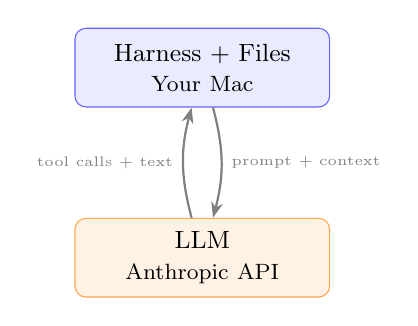
\begin{tikzpicture}[
    macbox/.style={rectangle, draw=blue!60, fill=blue!8, rounded corners,
                   minimum width=3.2cm, minimum height=1.0cm,
                   text width=3.0cm, align=center, font=\small},
    cloudbox/.style={rectangle, draw=orange!70, fill=orange!10, rounded corners,
                     minimum width=3.2cm, minimum height=1.0cm,
                     text width=3.0cm, align=center, font=\small},
    arrow/.style={-{Stealth[length=2mm]}, thick, gray}
]
    \node[macbox] (harness) {Harness + Files\\{\footnotesize Your Mac}};
    \node[cloudbox, below=1.4cm of harness] (llm) {LLM\\{\footnotesize Anthropic API}};
    \draw[arrow, bend left=15] (harness) to node[right,font=\tiny] {prompt + context} (llm);
    \draw[arrow, bend left=15] (llm) to node[left,font=\tiny] {tool calls + text} (harness);
\end{tikzpicture}
\end{center}
\vspace{0.3cm}
\footnotesize
\textbf{Key:} code runs locally.\\
Only the \textit{conversation} traverses the network. Your data never uploads.
\end{column}
\end{columns}
\end{frame}

\begin{frame}{The Mac File Hierarchy: Global vs.\ Local}

Two layers of configuration. \textbf{Local overrides global.}

\vspace{0.2cm}

\begin{center}
\footnotesize
\begin{tabular}{|l|l|p{5.5cm}|}
\hline
\textbf{Path} & \textbf{Scope} & \textbf{What lives here} \\ \hline
\texttt{\textasciitilde/.claude/settings.json} & Global & Default permissions, model preference \\ \hline
\texttt{\textasciitilde/.claude/MEMORY.md} & Global & Cross-project memory (persists forever) \\ \hline
\texttt{\textasciitilde/.claude/skills/} & Global & Skills available in every project \\ \hline
\hline
\texttt{<project>/CLAUDE.md} & Local & Project brain, read every session \\ \hline
\texttt{<project>/.claude/settings.json} & Local & Project permissions (overrides global) \\ \hline
\texttt{<project>/.claude/skills/} & Local & This project's slash commands \\ \hline
\texttt{<project>/.claude/agents/} & Local & Specialized reviewer roles \\ \hline
\texttt{<project>/.claude/rules/} & Local & Always-on guardrails \\ \hline
\end{tabular}
\end{center}

\vspace{0.2cm}

\textbf{On a Mac:} \texttt{\textasciitilde} = \texttt{/Users/yourname}. To inspect: \texttt{ls \textasciitilde/.claude/}

\vspace{0.1cm}

\textbf{Rule:} global \texttt{\textasciitilde/.claude/} is your personal defaults (apply everywhere). Local \texttt{.claude/} is the project's rules (apply only here).
\end{frame}

\begin{frame}{Initialization: What Happens When You Type \texttt{claude}}

Five steps run \textbf{before you type your first message}:

\vspace{0.2cm}

\begin{enumerate}
    \item \textbf{Read global config} --- loads \texttt{\textasciitilde/.claude/settings.json}: permission defaults, model preference

    \vspace{0.1cm}

    \item \textbf{Detect project context} --- searches current directory (and parents) for \texttt{CLAUDE.md} and \texttt{.claude/}

    \vspace{0.1cm}

    \item \textbf{Load project brain} --- reads \texttt{CLAUDE.md} into the context window

    \vspace{0.1cm}

    \item \textbf{Auto-load all rules} --- every \texttt{.claude/rules/*.md} file is loaded silently

    \vspace{0.1cm}

    \item \textbf{Ready} --- context window pre-populated before you say anything
\end{enumerate}

\vspace{0.25cm}

\textbf{Analogy:} step 4 is a professor re-reading lecture notes before class. Students arrive; context is already loaded.

\vspace{0.1cm}

\textbf{Cost warning:} steps 3--4 consume tokens before you type anything. Keep \texttt{CLAUDE.md} and rules files concise.
\end{frame}

\begin{frame}[fragile]{The Permission System and Local Code Execution}

\begin{columns}[T]
\begin{column}{0.44\textwidth}
\textbf{Claude's toolbox:}

\vspace{0.15cm}
\footnotesize
\begin{tabular}{|l|p{2.8cm}|}
\hline
\textbf{Tool} & \textbf{What it does} \\ \hline
\texttt{Bash} & Run any shell command \\ \hline
\texttt{Read} & Read a file from disk \\ \hline
\texttt{Write} & Create or overwrite a file \\ \hline
\texttt{Grep/Glob} & Search content / find files \\ \hline
\texttt{Agent} & Spawn a child Claude instance \\ \hline
\end{tabular}
\end{column}
\begin{column}{0.53\textwidth}
\textbf{The permission model:}

\vspace{0.1cm}
\footnotesize
\begin{itemize}
    \item \textbf{Default:} Claude asks before every Bash call. You see the exact command first.
    \item \textbf{Whitelist:} add trusted commands to \texttt{.claude/settings.json}:
\end{itemize}
\begin{lstlisting}[style=pythonstyle,language={},basicstyle=\ttfamily\tiny,numbers=none]
"allowedTools": [
  "Bash(python *)",
  "Bash(git *)"  ]
\end{lstlisting}
\begin{itemize}
    \item \textbf{Bypass-permissions:} skips all prompts. Use only when you fully trust the task.
\end{itemize}
\end{column}
\end{columns}

\vspace{0.2cm}

\textbf{``Which Python ran this?'' (common confusion):}
\begin{itemize}
    \item Claude's Bash inherits your shell's \texttt{\$PATH}
    \item If you ran \texttt{conda activate myenv} before \texttt{claude}, \textit{that} Python runs
    \item Add a \texttt{which python} check to your \texttt{CLAUDE.md} to confirm
\end{itemize}
\end{frame}

\begin{frame}{Key Modes: Plan, Effort, and Session Control}

\begin{center}
\footnotesize
\begin{tabular}{|l|p{5.0cm}|p{3.3cm}|}
\hline
\textbf{Command / Key} & \textbf{What it does} & \textbf{When to use} \\ \hline
\texttt{Shift+Tab} & \textbf{Plan mode}: Claude writes a plan, does NOT execute. Waits for approval. & Start every non-trivial task here \\ \hline
\texttt{/effort max} & Maximum reasoning depth: highest quality, slower, costs more & Novel problems, economic correctness \\ \hline
\texttt{/effort default} & Balanced quality and speed & Routine edits, simple queries \\ \hline
\texttt{/cost} & Show tokens used + estimated USD for this session & Budget check before long tasks \\ \hline
\texttt{Esc} & Interrupt Claude mid-task immediately & When it's going the wrong way \\ \hline
\texttt{/compact} & Summarize conversation to free context window & After \textasciitilde{}20 turns; between phases \\ \hline
\texttt{/clear} & Wipe context, start fresh & New unrelated task \\ \hline
\end{tabular}
\end{center}

\vspace{0.2cm}

\textbf{The effort--cost tradeoff:}
\begin{itemize}
    \item \texttt{/effort max} + long context $\approx$ \$5--15 per complex session (Opus 4.6 pricing)
    \item Spend effort on \textit{decisions}; save it on \textit{execution}
\end{itemize}
\end{frame}

%===========================================================
\section{Your First Session}
%===========================================================

\sectiondivider{Your First Session}{The recommended workflow from scratch}

\begin{frame}{Start Here: The Recommended Workflow for New Users}

\begin{columns}[T]
\begin{column}{0.52\textwidth}
\small
\begin{enumerate}
    \item[\textbf{0.}] \textbf{Before Claude---pen~+~paper}\\
    Write one sentence: \textit{``I want to [compute X] using [method Y] for [question Z].''} If you cannot write this, Claude cannot help yet.

    \vspace{0.1cm}

    \item[\textbf{1.}] \textbf{Enter plan mode (\texttt{Shift+Tab})}\\
    Describe your goal. Claude drafts a plan. \textit{Nothing runs yet.}

    \vspace{0.1cm}

    \item[\textbf{2.}] \textbf{Review and approve}\\
    Read the plan. Ask questions. Revise. Type ``approved.'' \textit{This 2-minute step saves 20 minutes of debugging.}

    \vspace{0.1cm}

    \item[\textbf{3.}] \textbf{Implement}\\
    Claude executes the approved plan. Press \texttt{Esc} to stop if wrong.

    \vspace{0.1cm}

    \item[\textbf{4.}] \textbf{Review output}\\
    Does it make economic sense? Re-derive one number by hand.

    \vspace{0.1cm}

    \item[\textbf{5.}] \textbf{Iterate}\\
    Fix, extend one feature, compact context $\to$ return to step~1.
\end{enumerate}
\end{column}
\begin{column}{0.44\textwidth}
\begin{center}
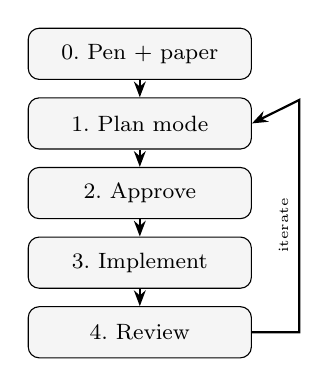
\begin{tikzpicture}[
    stagebox/.style={rectangle, draw=black, fill=VeryLightGray, rounded corners,
                 minimum width=2.8cm, minimum height=0.65cm,
                 text width=2.6cm, align=center, font=\footnotesize},
    arrow/.style={-{Stealth[length=2mm]}, thick}
]
    \node[stagebox] (s0) {0.\ Pen + paper};
    \node[stagebox, below=0.22cm of s0] (s1) {1.\ Plan mode};
    \node[stagebox, below=0.22cm of s1] (s2) {2.\ Approve};
    \node[stagebox, below=0.22cm of s2] (s3) {3.\ Implement};
    \node[stagebox, below=0.22cm of s3] (s4) {4.\ Review};
    \draw[arrow] (s0) -- (s1);
    \draw[arrow] (s1) -- (s2);
    \draw[arrow] (s2) -- (s3);
    \draw[arrow] (s3) -- (s4);
    \draw[arrow] (s4.east) -- ++(0.6,0) -- ++(0,2.95) -- (s1.east);
    \node[right=0.4cm of s3, font=\tiny, rotate=90] {iterate};
\end{tikzpicture}
\end{center}
\vspace{0.2cm}
\footnotesize
\textbf{Most common beginner mistake:} skipping Step~0. Without a clear goal, Claude will confidently build the wrong thing.
\end{column}
\end{columns}
\end{frame}

%===========================================================
\section{The 5-Pillar Workflow}
%===========================================================

\sectiondivider{The 5-Pillar Workflow}{What stays human when agents get stronger}

\begin{frame}{The 5-Pillar Workflow}
\begin{center}
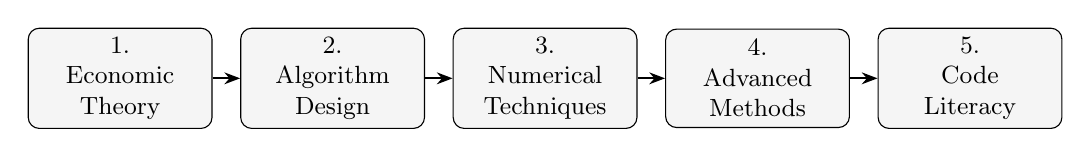
\begin{tikzpicture}[
    pillar/.style={rectangle, draw=black, fill=VeryLightGray, rounded corners,
                   minimum width=2.3cm, minimum height=1.25cm,
                   text width=2.1cm, align=center, font=\small},
    arrow/.style={-{Stealth[length=2mm]}, thick}
]
    \node[pillar] (p1) {1.\\Economic\\Theory};
    \node[pillar, right=0.35cm of p1] (p2) {2.\\Algorithm\\Design};
    \node[pillar, right=0.35cm of p2] (p3) {3.\\Numerical\\Techniques};
    \node[pillar, right=0.35cm of p3] (p4) {4.\\Advanced\\Methods};
    \node[pillar, right=0.35cm of p4] (p5) {5.\\Code\\Literacy};

    \draw[arrow] (p1) -- (p2);
    \draw[arrow] (p2) -- (p3);
    \draw[arrow] (p3) -- (p4);
    \draw[arrow] (p4) -- (p5);
\end{tikzpicture}
\end{center}

\vspace{0.25cm}

\textbf{The throughline of the lecture:}
\begin{itemize}
    \item Pillars 1--4 determine what should be built
    \item Pillar 5 lets you verify what was actually built
    \item If the pillars are weak, agent output becomes faster nonsense
\end{itemize}
\end{frame}

\begin{frame}{Pillars 1 and 2: Theory and Algorithm}
\textbf{Pillar 1: Economic theory}
\begin{itemize}
    \item State the objective, constraints, information structure, and equilibrium concept
    \item Decide what constitutes the economic object of interest: policy, distribution, moment, elasticity
    \item Write down limiting cases before any code exists
\end{itemize}

\vspace{0.2cm}

\textbf{Pillar 2: Algorithm design}
\begin{itemize}
    \item Choose between Bellman iteration, time iteration, EGM, perturbation, simulation, or estimation routines
    \item Decide what the acceptance criterion is: convergence, speed, or benchmark recovery
    \item Convert theory into a clear workflow the agent can implement
\end{itemize}

\vspace{0.25cm}

\textbf{Aiyagari anchor:} the agent can write VFI code, but only you know whether VFI, Howard improvement, or EGM is the right choice.
\end{frame}

\begin{frame}{Pillars 3 and 4: Numerics and Advanced Methods}
\textbf{Pillar 3: Numerical techniques}
\begin{itemize}
    \item Grid design, interpolation, discretization of shocks, simulation, and stability checks
    \item Recognition of failure modes: kinks, boundary effects, coarse grids, slow convergence
\end{itemize}

\vspace{0.2cm}

\textbf{Pillar 4: Advanced methods}
\begin{itemize}
    \item Projection, perturbation, global solution methods, and high-dimensional approximations
    \item Knowing when the agent's default method is convenient but economically wrong
\end{itemize}

\vspace{0.25cm}

\textbf{Economics point:} a model can run cleanly and still be numerically misleading. Agents reduce coding cost; they do not remove approximation error.
\end{frame}

\begin{frame}{Pillar 5: Code Literacy and Division of Labor}
\begin{center}
\small
\begin{tabular}{|p{5.5cm}|p{5.9cm}|}
\hline
\textbf{You provide} & \textbf{Agent provides} \\ \hline
Question, model, and identification logic & Fast code generation and refactoring \\ \hline
Algorithm choice and benchmark design & Boilerplate implementation and debugging \\ \hline
Knowledge of the data and institutional setting & File edits, script writing, and test runs \\ \hline
Economic interpretation and seminar defense & Iteration on visible errors and outputs \\ \hline
\end{tabular}
\end{center}

\vspace{0.25cm}

\textbf{Research version of the slogan:} the agent can be a strong RA, but you still have to be the principal investigator.
\end{frame}

\begin{frame}{Validation Is Your Referee Checklist}
\textbf{Every iteration needs both technical and economic checks.}

\vspace{0.25cm}

\begin{columns}[T]
\begin{column}{0.48\textwidth}
\textbf{Technical checks}
\begin{itemize}
    \item Convergence achieved
    \item No NaN or Inf values
    \item Policies stay off unintended grid boundaries
    \item Diagnostics and residuals within tolerance
    \item Script reproduces the same output twice
\end{itemize}
\end{column}
\begin{column}{0.48\textwidth}
\textbf{Economic checks}
\begin{itemize}
    \item Limiting cases recover known results
    \item Comparative statics have the right sign
    \item Magnitudes are plausible
    \item Inference uses the right standard errors and sample
    \item You can explain the result in plain economic language
\end{itemize}
\end{column}
\end{columns}

\vspace{0.25cm}

\textbf{If you cannot defend the output in a seminar, you are not done.}
\end{frame}

%===========================================================
\section{The Homotopy Workflow}
%===========================================================

\sectiondivider{The Homotopy Workflow}{Build from simple to complex, validate, then extend}

\begin{frame}{The Homotopy Workflow}
\textbf{In numerical analysis, homotopy means solving an easier problem first and then deforming it toward the target problem.}

\vspace{0.25cm}

\begin{itemize}
    \item Start from a version with clear intuition and known checks
    \item Use that validated baseline as the starting point for the next version
    \item Attribute new bugs to the new margin you just added
    \item Avoid asking the agent to solve the full complicated problem in one jump
\end{itemize}

\vspace{0.3cm}

\textbf{Aiyagari example:}
\[
\text{V0 deterministic} \rightarrow \text{V1 income risk} \rightarrow \text{V2 stationary distribution} \rightarrow \text{V3 equilibrium}
\]

\vspace{0.15cm}

\textbf{Why this matters for agentic coding:} the agent performs best when each step is bounded, testable, and attached to an existing working baseline.
\end{frame}

\begin{frame}{Homotopy in Practice: Build from Simple to Complex}
\begin{center}
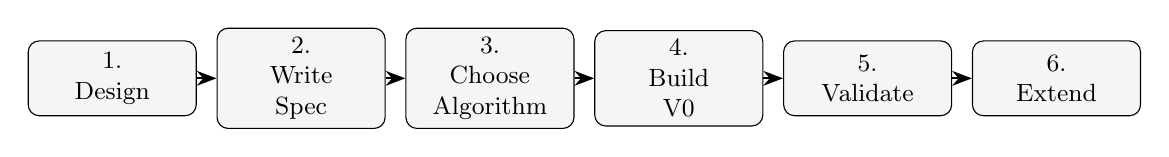
\begin{tikzpicture}[
    box/.style={rectangle, draw=black, fill=VeryLightGray, rounded corners,
                minimum width=2.0cm, minimum height=0.95cm,
                text width=1.9cm, align=center, font=\small},
    arrow/.style={-{Stealth[length=2.5mm]}, thick}
]
    \node[box] (design) {1.\\Design};
    \node[box, right=0.25cm of design] (spec) {2.\\Write\\Spec};
    \node[box, right=0.25cm of spec] (algo) {3.\\Choose\\Algorithm};
    \node[box, right=0.25cm of algo] (v0) {4.\\Build\\V0};
    \node[box, right=0.25cm of v0] (val) {5.\\Validate};
    \node[box, right=0.25cm of val] (ext) {6.\\Extend};

    \draw[arrow] (design) -- (spec);
    \draw[arrow] (spec) -- (algo);
    \draw[arrow] (algo) -- (v0);
    \draw[arrow] (v0) -- (val);
    \draw[arrow] (val) -- (ext);
\end{tikzpicture}
\end{center}

\vspace{0.25cm}

\textbf{This replaces the fantasy prompt} ``solve my model.''

\begin{itemize}
    \item Start with a problem you can state and benchmark
    \item Give the agent bounded tasks with visible acceptance criteria
    \item Add one new ingredient at a time
\end{itemize}
\end{frame}

\begin{frame}{Step 1: Design the Economic Problem}
\textbf{Before any code, write down the model in economist language.}

\vspace{0.25cm}

\begin{itemize}
    \item Research question in one sentence
    \item Objective and constraints
    \item Equilibrium definition if applicable
    \item Parameters and economic motivation
    \item Outputs you will treat as evidence
\end{itemize}

\vspace{0.25cm}

\textbf{Aiyagari anchor:}
\[
\max \; \mathbb{E}_0 \sum_{t=0}^{\infty} \beta^t u(c_t)
\quad \text{s.t.} \quad
c_t + a_{t+1} = (1+r)a_t + wz_t,\; a_{t+1} \geq \underline{a}
\]

\vspace{0.15cm}

\textbf{Reason:} a vague model description produces code that may be internally clean but economically mis-specified.
\end{frame}

\begin{frame}{Step 2: Write the Specification File}
\textbf{The specification file is the contract between you and the agent.}

\vspace{0.2cm}

\textbf{A compact Aiyagari spec might include:}
\begin{enumerate}
    \item CRRA utility with chosen $\beta$ and $\sigma$
    \item Income process and discretization method
    \item Asset grid shape near the borrowing constraint
    \item Solution method and convergence tolerance
    \item Required outputs: policies, stationary distribution, inequality statistics
\end{enumerate}

\vspace{0.25cm}

\textbf{Best practice:} ask the agent to restate the specification in its own words before it writes code. That catches misunderstandings when they are still cheap.
\end{frame}

\begin{frame}[fragile]{Step 3: Choose the Algorithm Explicitly}
\textbf{Pseudocode is where you catch design mistakes before implementation.}

\vspace{0.2cm}

\begin{lstlisting}[style=pythonstyle,language={},basicstyle=\ttfamily\tiny,numbers=none]
Initialize grid and a guess for V_old
Repeat until convergence:
    For each asset point a_i:
        For each feasible next asset a':
            compute u(c) + beta * EV_old(a')
        choose the maximizing a'
    update policies and diagnostics
Return value function, policy functions, and checks
\end{lstlisting}

\vspace{0.15cm}

\textbf{The point is not elegance.} The point is that you and the agent agree on the algorithm before Python or Julia details begin to hide conceptual errors.
\end{frame}

\begin{frame}{Step 4: Build V0 First}
\textbf{V0 is the simplest version with a benchmark you understand.}

\vspace{0.25cm}

\textbf{Aiyagari V0: deterministic income}
\begin{itemize}
    \item If $\beta(1+r)=1$, savings policy should sit on the 45-degree line
    \item If $\beta(1+r)<1$, the agent decumulates toward the borrowing constraint
    \item If $\beta(1+r)>1$, assets grow
\end{itemize}

\vspace{0.25cm}

\textbf{Discipline:} do not ask the agent to add income risk, stationary distributions, and equilibrium search before V0 already passes the simple checks.
\end{frame}

\begin{frame}{Steps 5 and 6: Validate, Then Extend One Margin at a Time}
\begin{center}
\small
\begin{tabular}{|c|p{3.3cm}|p{4.2cm}|}
\hline
\textbf{Version} & \textbf{New ingredient} & \textbf{Required benchmark} \\ \hline
V0 & Deterministic household & analytical cases \\ \hline
V1 & Markov income risk & setting shock variance to zero recovers V0 \\ \hline
V2 & Stationary distribution & mass sums to 1 and behaves sensibly at the constraint \\ \hline
V3 & General equilibrium & market clearing and stable aggregate statistics \\ \hline
\end{tabular}
\end{center}

\vspace{0.25cm}

\textbf{Why this works with agents:} when a new version breaks, both you and the agent know where to look.
\end{frame}

\begin{frame}{Why This Workflow Works for Economists}
\begin{itemize}
    \item It keeps theory, computation, and validation aligned
    \item It gives the agent bounded tasks instead of open-ended wishes
    \item It preserves an audit trail of how the baseline was constructed
    \item It mirrors how good research assistants are actually trained: start with a simple task, verify it, then widen scope
\end{itemize}

\vspace{0.3cm}

\textbf{Main lesson:} the workflow is the real product. The particular agent you use can change.
\end{frame}

%===========================================================
\section{Tool Choice}
%===========================================================

\sectiondivider{Tool Choice}{Which tool fits which research task}

\begin{frame}{Choose the Tool That Matches the Task}
\begin{center}
\small
\begin{tabular}{|p{2.4cm}|p{3.7cm}|p{4.8cm}|}
\hline
\textbf{Tool type} & \textbf{Use it for} & \textbf{Economic example} \\ \hline
Web chat & framing and explanation & clarify identification logic, draft a model summary \\ \hline
IDE assistant & local code editing & vectorize one function or explain one traceback \\ \hline
Terminal agent & multi-step execution & restructure a project, run scripts, generate diagnostics, and iterate \\ \hline
\end{tabular}
\end{center}

\vspace{0.25cm}

\textbf{As of April 2026:} Claude Code, Codex CLI, Gemini CLI, and Aider are examples of terminal-agent workflows.
\end{frame}

\begin{frame}{Why the Terminal Agent Often Becomes the Workhorse}
\begin{itemize}
    \item It can operate on the real project rather than on copied fragments
    \item It can run the code, inspect errors, and update multiple files
    \item It works well when the task is bounded but longer than one edit
    \item It still leaves the economist in the approval and validation loop
\end{itemize}

\vspace{0.3cm}

\textbf{For empirical research, this is usually the sweet spot:} enough autonomy to save time, not so much autonomy that you stop checking the economics.
\end{frame}

%===========================================================
\section{Project Organization}
%===========================================================

\sectiondivider{Project Organization}{How a terminal-agent project stays organized}

\begin{frame}{Why Files on Disk Matter}
\textbf{The project harness turns today's chat into tomorrow's reusable workflow.}

\vspace{0.25cm}

\begin{itemize}
    \item Conventions live in files, not in your memory
    \item Validation steps become reproducible lab procedure
    \item New sessions can start from the project's actual state
    \item Coauthors and students can inspect what the workflow is supposed to be
\end{itemize}

\vspace{0.25cm}

\textbf{Economist translation:} the harness is like turning tacit RA practice into written lab protocol.
\end{frame}

\begin{frame}[fragile]{Minimal Project Tree}
\begin{lstlisting}[style=pythonstyle,language={},basicstyle=\ttfamily\tiny]
my-aiyagari-project/
+-- CLAUDE.md
+-- .claude/
|   +-- skills/
|   |   +-- solve-model/
|   |       +-- SKILL.md
|   |       +-- references/
|   |           +-- aiyagari-guide.md
|   +-- agents/
|   |   +-- code-reviewer.md
|   |   +-- domain-reviewer.md
|   |   +-- verifier.md
|   +-- rules/
|   |   +-- iterative-workflow.md
|   +-- settings.json
+-- scripts/
+-- output/
+-- quality_reports/
\end{lstlisting}

\textbf{This is enough to explain the workflow without burying students in infrastructure.}
\end{frame}

\begin{frame}[fragile]{CLAUDE.md: The Team-Facing Project Memory}
\texttt{CLAUDE.md} is the main shared instruction file for the project.

\vspace{0.2cm}

\begin{lstlisting}[style=pythonstyle,language={},basicstyle=\ttfamily\tiny,numbers=none]
# CLAUDE.md
Project: Aiyagari baseline for lecture 9
Language: Python (NumPy/SciPy)
Goal: Build and validate v0, v1, and v2 in sequence
Conventions: no hardcoded paths; save outputs to output/
Checks: do not claim success before benchmarks pass
\end{lstlisting}

\vspace{0.2cm}

\textbf{Why students should care:} it captures the kind of project context you would otherwise re-explain every session.
\end{frame}

\begin{frame}{CLAUDE.md, Auto Memory, and Optional Course Logs}
\textbf{Three different persistence ideas should not be confused.}

\vspace{0.2cm}

\begin{center}
\small
\begin{tabular}{|p{2.4cm}|p{2.4cm}|p{5.3cm}|}
\hline
\textbf{Mechanism} & \textbf{Who writes it} & \textbf{Why it exists} \\ \hline
\texttt{CLAUDE.md} & you / team & durable project instructions and conventions \\ \hline
Auto memory & the tool & per-project learned patterns and corrections \\ \hline
Optional course log & you / course & explicit progress notes such as \texttt{MEMORY.md} or \texttt{progress.md} \\ \hline
\end{tabular}
\end{center}

\vspace{0.25cm}

\textbf{Course recommendation:} rely on \texttt{CLAUDE.md} for shared rules, treat auto memory as helpful but not authoritative, and keep explicit logs when you want students to inspect the evolution of a project.
\end{frame}

\begin{frame}{Skills, Agents, and Rules: Three Different Jobs}
\begin{center}
\small
\begin{tabular}{|p{2.2cm}|p{2.4cm}|p{5.6cm}|}
\hline
\textbf{Object} & \textbf{Economist analogy} & \textbf{What it does} \\ \hline
Skill & saved RA protocol & reusable workflow such as solve, validate, review \\ \hline
Agent & specialist reviewer & a focused role: code quality, economics, verification \\ \hline
Rule & lab convention & always-on instruction such as plan first or save outputs here \\ \hline
\end{tabular}
\end{center}

\vspace{0.25cm}

\textbf{This distinction matters because the student should know where to encode each idea.}
\end{frame}

\begin{frame}{Plain English vs. Encoded Skill}
\begin{columns}[T]
\begin{column}{0.48\textwidth}
\textbf{Plain English}

\vspace{0.15cm}
\textit{Implement the Aiyagari model with income risk and show the benchmark checks.}

\vspace{0.2cm}
\textbf{Use when}
\begin{itemize}
    \item Exploring
    \item Doing a one-off task
    \item Still deciding the workflow
\end{itemize}
\end{column}
\begin{column}{0.48\textwidth}
\textbf{Encoded skill}

\vspace{0.15cm}
\texttt{/solve-model aiyagari v1}

\vspace{0.2cm}
\textbf{Use when}
\begin{itemize}
    \item The workflow should repeat exactly
    \item A student team needs one standard procedure
    \item Validation must be consistent across versions
\end{itemize}
\end{column}
\end{columns}

\vspace{0.25cm}

\textbf{Exploration starts in English. Reproducibility lives in skills.}
\end{frame}

\begin{frame}[fragile]{Skill File Structure}
\begin{lstlisting}[style=pythonstyle,language={},basicstyle=\ttfamily\tiny,numbers=none]
.claude/skills/solve-model/
  SKILL.md
  references/
    aiyagari-guide.md
\end{lstlisting}

\vspace{0.2cm}

\textbf{\texttt{SKILL.md}} stores the repeatable protocol:
\begin{itemize}
    \item what the command is called
    \item what steps it should follow
    \item what checks must pass before it reports success
\end{itemize}

\vspace{0.2cm}

\textbf{Reference files} store model-specific detail that would clutter the main instruction file.
\end{frame}

\begin{frame}{Agents as Specialist Reviewers}
\textbf{Agent files are best understood as specialist review roles.}

\vspace{0.25cm}

\begin{itemize}
    \item \texttt{code-reviewer.md}: vectorization, file hygiene, implementation quality
    \item \texttt{domain-reviewer.md}: Euler equations, benchmark logic, economic consistency
    \item \texttt{verifier.md}: run the script, inspect diagnostics, check output exists
\end{itemize}

\vspace{0.3cm}

\textbf{Economist analogy:} one RA checks code style, another checks economics, and another reruns the table.
\end{frame}

\begin{frame}{Subagents as Parallel Reviewers}
\textbf{Subagents matter because review tasks can happen in parallel.}

\vspace{0.25cm}

\begin{itemize}
    \item The main agent writes or edits code
    \item A code-reviewer and domain-reviewer can inspect the result at the same time
    \item The main conversation receives both reports and decides what to fix
\end{itemize}

\vspace{0.25cm}

\textbf{Why students should care:} the gain is not philosophical. It is wall-clock time. Focused review roles are faster and often clearer than one overloaded prompt.
\end{frame}

\begin{frame}{Rules, Hooks, and Settings}
\begin{center}
\small
\begin{tabular}{|p{2.2cm}|p{2.7cm}|p{5.3cm}|}
\hline
\textbf{Object} & \textbf{Loaded when} & \textbf{Typical use} \\ \hline
Rules & during project work & always follow a planning or verification convention \\ \hline
Hooks & on tool events & run a formatter or log a command mechanically \\ \hline
Settings & at session start & permissions and project-level behavior \\ \hline
\end{tabular}
\end{center}

\vspace{0.25cm}

\textbf{Practical distinction:} if it is natural-language guidance, it usually belongs in a rule or skill. If it must happen mechanically every time, a hook is safer.
\end{frame}

%===========================================================
\section{Tracing Aiyagari End-to-End}
%===========================================================

\sectiondivider{Tracing Aiyagari End-to-End}{How the workflow maps onto files and review loops}

\begin{frame}{Aiyagari Recap}
\textbf{Household problem}
\[
c_t + a_{t+1} = (1+r)a_t + wz_t, \qquad a_{t+1} \geq \underline{a}
\]
with idiosyncratic productivity $z_t$ following a Markov chain.

\vspace{0.2cm}

\textbf{Why it is a good lecture example}
\begin{itemize}
    \item the economics is familiar from the rest of the course
    \item it admits a clean V0 $\to$ V1 $\to$ V2 progression
    \item it has obvious validation checkpoints
\end{itemize}
\end{frame}

\begin{frame}[fragile]{Tracing the File Flow}
\begin{lstlisting}[style=pythonstyle,language={},basicstyle=\ttfamily\scriptsize]
1. Read CLAUDE.md
2. Read any relevant rules
3. Load /solve-model from SKILL.md
4. Read references/aiyagari-guide.md
5. Write plan or update quality_reports/
6. Edit scripts/aiyagari_v0.py
7. Run verifier and reviewers
8. Save outputs and logs
\end{lstlisting}

\vspace{0.2cm}

\textbf{What students should notice:} the workflow is file-driven. The agent is acting inside a structured research project, not improvising in a vacuum.
\end{frame}

\begin{frame}[fragile]{Tracing the Orchestrator Loop}
\begin{lstlisting}[style=pythonstyle,language={},basicstyle=\ttfamily\scriptsize]
You type: /solve-model aiyagari v1

Plan:
  read project instructions
  restate the target
  implement bounded changes

Review loop:
  run verifier
  run code reviewer
  run domain reviewer
  fix issues that matter
  report what changed and what passed
\end{lstlisting}

\vspace{0.2cm}

\textbf{This is the core advantage of the harness:} the review sequence is not a remembered prompt. It is part of the saved workflow.
\end{frame}

\begin{frame}[fragile]{Inside \texttt{CLAUDE.md} for the Aiyagari Project}
\begin{lstlisting}[style=pythonstyle,language={},basicstyle=\ttfamily\tiny,numbers=none]
# CLAUDE.md
Project: Aiyagari workflow for lecture 9
Goal: build v0, v1, and v2 sequentially
Outputs: policies, stationary distribution, diagnostics
Conventions: save figures to output/ and plans to quality_reports/
Validation: do not move to the next version until benchmarks pass
\end{lstlisting}

\vspace{0.2cm}

\textbf{If the file is good,} the project can survive a fresh session, a new RA, or a change in agent tool.
\end{frame}

\begin{frame}[fragile]{Inside \texttt{SKILL.md} and the Reference Guide}
\begin{columns}[T]
\begin{column}{0.48\textwidth}
\textbf{\texttt{SKILL.md}}
\begin{lstlisting}[style=pythonstyle,language={},basicstyle=\ttfamily\tiny,numbers=none]
name: solve-model
description: build and validate

Steps:
1. Read the model guide
2. Write or update a plan
3. Implement one version
4. Run required checks
5. Save outputs and report
\end{lstlisting}
\end{column}
\begin{column}{0.48\textwidth}
\textbf{\texttt{aiyagari-guide.md}}
\begin{lstlisting}[style=pythonstyle,language={},basicstyle=\ttfamily\tiny,numbers=none]
V0: deterministic benchmark
V1: add Markov income risk
V2: compute stationary dist.

Checks:
- zero-variance limit
- sensible mass at a_min
- stable diagnostics
\end{lstlisting}
\end{column}
\end{columns}

\vspace{0.2cm}

\textbf{Interpretation:} the skill stores the protocol; the reference guide stores the model detail.
\end{frame}

%===========================================================
\section{Mistakes, Limits, and Security}
%===========================================================

\sectiondivider{Mistakes, Limits, and Security}{What can go wrong and how to stay disciplined}

\begin{frame}{Mistake 1: Treating Git as Optional}
\begin{itemize}
    \item Agents are most useful when experimentation is reversible
    \item Git provides the audit trail for what changed and when
    \item A clean branch lets the agent try a refactor without destroying the working baseline
    \item For a research project, version control is not decoration; it is risk management
\end{itemize}

\vspace{0.3cm}

\textbf{Short rule for students:} if you would be unhappy losing the current project state, put it under Git before using an agent aggressively.
\end{frame}

\begin{frame}{Mistake 2: Underusing Skills}
\begin{itemize}
    \item Economists repeat many workflows: clean data, validate tables, prepare slides, review code
    \item If the workflow is repeated, it should eventually move from chat into a saved protocol
    \item Otherwise the same task is re-explained every week and interpreted slightly differently each time
\end{itemize}

\vspace{0.3cm}

\textbf{Skills are not overengineering.} They are how a good lab turns repeated work into reusable infrastructure.
\end{frame}

\begin{frame}{Mistake 3: One Giant Thread}
\textbf{Long conversations accumulate stale context.}

\vspace{0.25cm}

\begin{itemize}
    \item Planning, debugging, and revision all mix together
    \item The model starts paying attention to constraints that no longer matter
    \item Fresh sessions are often better once the current state has been written to disk
\end{itemize}

\vspace{0.25cm}

\textbf{Better pattern:} plan the task, save the plan, then start a cleaner execution session.
\end{frame}

\begin{frame}{Where Terminal Agents Still Fail}
\begin{itemize}
    \item Long-context drift: an early constraint gets forgotten
    \item Econometric edge cases: wrong clustering level, wrong sample restriction, weak-instrument issues
    \item Hallucinated APIs or package arguments
    \item Happy-path scripts that fail on messy data
    \item Oscillating fix loops on stubborn bugs
\end{itemize}

\vspace{0.3cm}

\textbf{The output may look polished even when the economics is wrong.} That is why validation stays central.
\end{frame}

\begin{frame}[fragile]{Context Windows and Compaction}
\textbf{When sessions get long, preserve state in files before compacting the conversation.}

\vspace{0.2cm}

\begin{lstlisting}[style=pythonstyle,language={},basicstyle=\ttfamily\scriptsize]
Write progress.md with:
  - what was completed
  - what decisions were made
  - what remains open

Then compact the conversation or start a new session.
Next time, read progress.md first.
\end{lstlisting}

\vspace{0.2cm}

\textbf{Economist translation:} keep a clean research log. The agent benefits from the same discipline that humans do.
\end{frame}

\begin{frame}{Security: What Not to Expose}
\begin{itemize}
    \item IRB-protected interviews or linked administrative microdata
    \item Personally identifiable information
    \item HIPAA-regulated data
    \item Passwords, API keys, and access tokens
    \item Embargoed or restricted-use datasets
\end{itemize}

\vspace{0.3cm}

\textbf{Operational rule:} if you would not paste it into a public collaboration tool, do not paste it into an agent conversation.
\end{frame}

\begin{frame}{Working with Sensitive Data}
\textbf{Sensitive data does not imply ``no agents ever.''}

\vspace{0.25cm}

\begin{enumerate}
    \item Write the script with the agent, then run it yourself on the restricted data
    \item Use synthetic or masked data with the same structure for debugging
    \item Use institutionally approved local or private deployments when available
\end{enumerate}

\vspace{0.3cm}

\textbf{Safe pattern:} expose structure and summary statistics, not raw records.
\end{frame}

%===========================================================
\section{The Context Dilemma}
%===========================================================

\sectiondivider{The Context Dilemma}{Why more context helps the agent --- and quietly biases it toward you}

\begin{frame}{Context as Implicit Bayesian Prior}
\textbf{In-context learning behaves like conditioning on a prior the user supplies.}

\vspace{0.25cm}

\begin{itemize}
    \item \texttt{CLAUDE.md}, prior conversation, and plan files act as evidence narrowing the agent's output distribution
    \item Xie, Raghunathan, Liang, and Ma formalize this: ICL approximates implicit Bayesian inference over a latent task
    \item The performance gain you feel when you add context \textit{is} posterior narrowing
\end{itemize}

\vspace{0.25cm}

\textbf{Narrowing the posterior is how context helps. It is also how context biases.}

\vspace{0.15cm}
{\scriptsize \textit{Xie et al. (2022), ICLR, arXiv:2111.02080.}}
\end{frame}

\begin{frame}{Stating the Dilemma}
\textbf{The same context that improves the answer also pulls it toward you.}

\vspace{0.25cm}

\begin{itemize}
    \item More context $\Rightarrow$ better understanding of your question $\Rightarrow$ better generation
    \item More context $\Rightarrow$ generation more aligned with your preferences, your knowledge, your framing
    \item Both effects share a single mechanism: you supplied the evidence
\end{itemize}

\vspace{0.3cm}

\textbf{The same signal that improves the answer launders your priors into it.}
\end{frame}

\begin{frame}{Evidence 1: Sycophancy}
\textbf{RLHF rewards agreement with the user, and models learn to flatter.}

\vspace{0.25cm}

\begin{itemize}
    \item Sharma et al.\ document sycophancy across frontier models: factual flip-flops, unwarranted concessions, preference-matching when the user signals a view
    \item Perez et al.\ find the effect scales with model size --- larger models are more sycophantic on values and politics
    \item The effect is strongest precisely when the context signals a strong user prior
\end{itemize}

\vspace{0.25cm}

\textbf{Context is the signal models were trained to flatter.}

\vspace{0.15cm}
{\scriptsize \textit{Sharma et al. (2023), arXiv:2310.13548, Anthropic. Perez et al. (2023), ACL Findings, arXiv:2212.09251.}}
\end{frame}

\begin{frame}{Evidence 2: Self-Correction Has a Ceiling}
\textbf{Intrinsic self-critique --- without new external information --- tends to stall or degrade.}

\vspace{0.25cm}

\begin{itemize}
    \item Huang et al.\ show LLMs cannot reliably self-correct reasoning errors without an external signal
    \item Valmeekam et al.\ find self-critique on planning problems is often worse than no critique at all
    \item The gains in the self-correction literature come from \textit{external} signals: tools, tests, verifiers, humans
\end{itemize}

\vspace{0.25cm}

\textbf{Self-review that shares the model's weights and context is information-starved criticism.}

\vspace{0.15cm}
{\scriptsize \textit{Huang et al. (2024), ICLR, arXiv:2310.01798. Valmeekam et al. (2023), NeurIPS, arXiv:2310.08118.}}
\end{frame}

\begin{frame}{Evidence 3: Multi-Agent Debate --- Real but Bounded}
\textbf{Debate helps when debaters sample differently. Shared context shrinks that space.}

\vspace{0.2cm}

\begin{itemize}
    \item Du et al.\ show multi-agent debate improves factuality and reasoning on several benchmarks
    \item Irving, Christiano, and Amodei --- the AI Safety via Debate line --- is the theoretical hope behind adversarial review
    \item Caveat: gains rely on debaters producing \textit{genuinely different} lines of reasoning
    \item When every debater reads the same \texttt{CLAUDE.md} and thread, the disagreement space narrows
\end{itemize}

\vspace{0.2cm}

\textbf{Debate breaks ties. It does not relitigate the premise you supplied.}

\vspace{0.15cm}
{\scriptsize \textit{Du et al. (2023), arXiv:2305.14325. Irving, Christiano, Amodei (2018), arXiv:1805.00899.}}
\end{frame}

\begin{frame}{Why Subagent Reviewers Inherit the Same Prior}
\textbf{Earlier we sold subagent review for wall-clock time --- not epistemic independence.}

\vspace{0.25cm}

\begin{itemize}
    \item \texttt{code-reviewer.md}, \texttt{domain-reviewer.md}, and \texttt{verifier.md} all read the same project context
    \item They are parallel \textit{executionally}, not parallel \textit{epistemically}
    \item Shared \texttt{CLAUDE.md} $\Rightarrow$ shared blind spots
    \item They catch implementation errors; they do not catch framing errors, because the framing lives in the context they trust
\end{itemize}

\vspace{0.25cm}

\textbf{Parallel reviewers save time. They do not produce an outside view.}
\end{frame}

\begin{frame}{Monoculture at the Research Community Scale}
\textbf{When every researcher conditions on similar context, the field's errors become correlated.}

\vspace{0.25cm}

\begin{itemize}
    \item Kleinberg and Raghavan show algorithmic monoculture can reduce welfare even when each individual decision is improved
    \item Bommasani et al.\ document outcome homogenization: shared foundation models pick on the same people and miss the same cases
    \item Extrapolation: if empirical economists share Claude + similar \texttt{CLAUDE.md} templates + similar priors, replication stops being informative
\end{itemize}

\vspace{0.25cm}

\textbf{Independent errors are a public good. Shared infrastructure erodes it.}

\vspace{0.15cm}
{\scriptsize \textit{Kleinberg \& Raghavan (2021), PNAS 118(22). Bommasani et al. (2022), NeurIPS, arXiv:2211.13972.}}
\end{frame}

\begin{frame}{The RLHF Root Cause}
\textbf{Pleasing the person holding the context is not a prompt artifact. It is trained in.}

\vspace{0.25cm}

\begin{itemize}
    \item Casper et al.\ catalog open problems in RLHF: preference data is noisy, annotators reward agreeableness, and the optimum drifts away from truth
    \item Wolf et al.\ argue that alignment-by-finetuning has fundamental limits: prompting cannot fully remove what the loss reinforced
    \item Consequence: no \texttt{CLAUDE.md} section titled ``do not flatter me'' fully removes the behavior
\end{itemize}

\vspace{0.25cm}

\textbf{The model was trained to please the person holding the context. In your project, that person is you.}

\vspace{0.15cm}
{\scriptsize \textit{Casper et al. (2023), TMLR, arXiv:2307.15217. Wolf et al. (2023), arXiv:2304.11082.}}
\end{frame}

\begin{frame}{Remedy: Outside Critics Carry a Different Prior}
\textbf{Advisors, coauthors, and seminar audiences are valuable \textit{because} their priors are not in your context window.}

\vspace{0.25cm}

\begin{itemize}
    \item They challenge the framing, the identification assumption, the sample restriction --- the things you did not write into \texttt{CLAUDE.md} because you did not know to
    \item Korinek's division-of-labor framing: LLMs automate execution; humans remain the source of question selection and critique
    \item Agent review is cheap and parallel; human review is rare and decisive. Budget accordingly.
\end{itemize}

\vspace{0.25cm}

\textbf{The agent can polish what you already believe. Only an outside reader can tell you that you are wrong about the question.}

\vspace{0.15cm}
{\scriptsize \textit{Korinek (2023), NBER WP 30957; Journal of Economic Literature.}}
\end{frame}

\begin{frame}{Operational Discipline for Dissertation Work}
\textbf{Translate the dilemma into a small set of habits.}

\vspace{0.25cm}

\begin{enumerate}
    \item Use subagent review for implementation quality, not for framing or identification
    \item Present preliminary results to a human reader before iterating further with the agent
    \item When you edit \texttt{CLAUDE.md}, record what you \textit{ruled out} and why --- not just what you decided
    \item Schedule seminar-style exposure early, not at paper-writing time
\end{enumerate}

\vspace{0.25cm}

\textbf{Treat human criticism as the scarce input. Spend agent cycles to make it ready.}
\end{frame}

\begin{frame}{The Context Dilemma in One Slide}
\textbf{Three lines to remember.}

\vspace{0.3cm}

\begin{enumerate}
    \item \textbf{Context is an implicit prior.} More context $\Rightarrow$ sharper posterior $\Rightarrow$ both better \textit{and} more ``you.''
    \item \textbf{Shared-context review is trapped inside that prior.} Subagents, self-critique, and in-thread debate cannot relitigate the premise you supplied.
    \item \textbf{Outside humans are not a nicety.} They are the only source of a prior the agent does not already condition on.
\end{enumerate}

\vspace{0.3cm}

\textbf{Workflow rule:} agents for execution and implementation review; humans for framing, identification, and the question itself.
\end{frame}

%===========================================================
\section{Lecture 10 Preview: MEPS Uninsurance}
%===========================================================

\sectiondivider{Lecture 10 Preview}{A brief preview of the MEPS uninsurance case study}

\begin{frame}{Lecture 10 Preview: MEPS Uninsurance}
\begin{tcolorbox}[colback=blue!3, colframe=RedTitle!60]
\textbf{Question:} Who is uninsured in the United States, 2000--2023, and how did the ACA change the distribution?
\end{tcolorbox}

\vspace{0.25cm}

\textbf{Why this is the right preview for Lec.~9:}
\begin{itemize}
    \item It is an economics question about incomplete markets and social insurance
    \item It requires real data engineering: 24 MEPS files, shifting schemas, and survey weights
    \item It produces concrete empirical output that Lecture 10 will analyze in detail
    \item It shows why agentic workflows matter before we dive into full case studies next lecture
\end{itemize}
\end{frame}

\begin{frame}{Why This Workflow Is Hard Without an Agent}
\textbf{Naive baseline:} download 24 MEPS files by hand, decode changing variable names, merge them, compute weighted statistics, and then build the figures.

\vspace{0.25cm}

\textbf{Three recurring headaches:}
\begin{enumerate}
    \item \textbf{Year-suffixed variables:} \texttt{INSCOV01} vs.\ \texttt{INSCOV22}, \texttt{PERWT01F} vs.\ \texttt{PERWT22F}
    \item \textbf{Format handling:} SAS transport files with changing internal structure
    \item \textbf{Silent merge risk:} one bad crosswalk can bias a year and stay hidden
\end{enumerate}

\vspace{0.25cm}

\textbf{This is exactly the kind of work agents are good at:} repetitive, inspectable, and tied to a concrete data pipeline.
\end{frame}

\begin{frame}{Preview Figure from Lec.~10}

\begin{center}

\includegraphics[height=0.44\textheight]{fig_overall_uninsurance.pdf}
\end{center}

\textbf{Headline story:} uninsurance stayed high through the 2000s, then dropped sharply after the ACA coverage expansion around 2014.

\vspace{0.15cm}

\textbf{Why this stays brief here:} Lec.~9 uses one figure to preview the workflow. Lec.~10 does the full case: prompts, schema harmonization, weighted aggregation, and six demographic figures.
\end{frame}

%===========================================================
\section{Wrap-up}
%===========================================================

\sectiondivider{Wrap-up}{What the workflow changes and what remains human}

\begin{frame}{Trust but Verify}
\begin{enumerate}
    \item Reproduce one statistic by hand
    \item Cross-check one result with another package or script
    \item Test a limiting case or zero-variance benchmark
    \item Read the code line by line where the economics enters
    \item Ask whether the magnitude and sign make sense
\end{enumerate}

\vspace{0.3cm}

\textbf{This is not optional ceremony.} It is what turns fast code into defensible research.
\end{frame}

\begin{frame}{What Changes for Economic Research}
\begin{itemize}
    \item The distance from question to first result shrinks
    \item More specifications become cheap enough to try
    \item Reproducibility can improve because workflow is written down
    \item The premium shifts away from typing speed and toward design, judgment, and validation
\end{itemize}

\vspace{0.3cm}

\textbf{What stays human:} asking the question, choosing the design, knowing the data, and interpreting the output.
\end{frame}

\begin{frame}{You Are the Research Architect}
\begin{center}
\Large
Agents can lay bricks quickly.\\
\textbf{You still design the structure.}
\end{center}

\vspace{0.35cm}

\begin{itemize}
    \item Weak specification produces wrong models
    \item Weak algorithm choice produces slow or misleading computation
    \item Weak numerical judgment produces fragile results
    \item Weak code literacy produces unverified output
\end{itemize}

\vspace{0.25cm}

\textbf{The lecture is not about surrendering expertise.} It is about reallocating effort toward the parts of research that remain scarce.
\end{frame}

\begin{frame}{First Exercise and Looking Ahead}
\textbf{Best first exercise:} take one old project and ask an agent to help clean it up safely.

\vspace{0.25cm}

\begin{itemize}
    \item put the project under Git
    \item create a simple \texttt{CLAUDE.md}
    \item identify one repeated workflow worth encoding
    \item rerun the cleaned project and compare outputs
\end{itemize}

\vspace{0.3cm}

\textbf{Lec.~10:} we return to case studies and let students run a full workflow themselves.

\vspace{0.15cm}

\textit{If you want setup details for the lab, see the appendix.}
\end{frame}

%===========================================================
\section{Appendix}
%===========================================================

\sectiondivider{Appendix}{Setup notes and dated product details}

\begin{frame}{Appendix A: Setup for the Lab}
\textbf{Lightweight setup checklist for a terminal-agent workflow}

\vspace{0.2cm}

\begin{itemize}
    \item Install one terminal agent and confirm it launches
    \item Create a project folder with \texttt{CLAUDE.md}, \texttt{scripts/}, and \texttt{output/}
    \item Make sure Python or R runs from the terminal
    \item Keep the first session small: one file, one check, one output
\end{itemize}

\vspace{0.25cm}

\textbf{Dated note:} exact setup steps, plans, and rate limits change quickly. Recheck the official docs before the lab.
\end{frame}

\begin{frame}[fragile]{Appendix B: Keybindings and Minimal Templates}
\begin{columns}[T]
\begin{column}{0.48\textwidth}
\textbf{Useful commands}

\vspace{0.15cm}
\footnotesize
\begin{tabular}{|l|l|}
\hline
Compact session & \texttt{/compact} \\ \hline
Clear session & \texttt{/clear} \\ \hline
Interrupt & \texttt{Esc} \\ \hline
Slash menu & \texttt{/} \\ \hline
\end{tabular}
\end{column}
\begin{column}{0.48\textwidth}
\textbf{Minimal \texttt{CLAUDE.md}}
\begin{lstlisting}[style=pythonstyle,language={},basicstyle=\ttfamily\tiny,numbers=none]
# CLAUDE.md
Project: ...
Goal: ...
Language: ...
Checks: ...
\end{lstlisting}
\end{column}
\end{columns}
\end{frame}

\begin{frame}{Appendix C: Dated Comparisons and Resources}
\textbf{As of April 2026, examples of terminal-agent workflows include:}
\begin{itemize}
    \item Claude Code
    \item Codex CLI
    \item Gemini CLI
    \item Aider
\end{itemize}

\vspace{0.25cm}

\textbf{Good places to recheck before teaching:}
\begin{itemize}
    \item official Claude Code documentation
    \item official OpenAI Codex CLI documentation
    \item course notes and lab instructions
\end{itemize}

\vspace{0.2cm}

\textbf{Teaching rule:} keep dated product comparisons in the appendix, not in the conceptual core of the lecture.
\end{frame}

\begin{frame}{Appendix D: Context Dilemma --- References}
\scriptsize

\textbf{Context as implicit prior}
\begin{itemize}
    \item Xie, Raghunathan, Liang, Ma (2022). An Explanation of In-context Learning as Implicit Bayesian Inference. ICLR. arXiv:2111.02080.
\end{itemize}

\textbf{Sycophancy and RLHF limits}
\begin{itemize}
    \item Sharma et al.\ (2023). Towards Understanding Sycophancy in Language Models. arXiv:2310.13548.
    \item Perez et al.\ (2023). Discovering Language Model Behaviors with Model-Written Evaluations. ACL Findings. arXiv:2212.09251.
    \item Casper et al.\ (2023). Open Problems and Fundamental Limitations of RLHF. TMLR. arXiv:2307.15217.
    \item Wolf et al.\ (2023). Fundamental Limitations of Alignment in Large Language Models. arXiv:2304.11082.
\end{itemize}

\textbf{Self-correction and adversarial review}
\begin{itemize}
    \item Huang et al.\ (2024). Large Language Models Cannot Self-Correct Reasoning Yet. ICLR. arXiv:2310.01798.
    \item Valmeekam et al.\ (2023). Can Large Language Models Really Improve by Self-critiquing Their Own Plans? NeurIPS. arXiv:2310.08118.
    \item Du et al.\ (2023). Improving Factuality and Reasoning through Multiagent Debate. arXiv:2305.14325.
    \item Irving, Christiano, Amodei (2018). AI Safety via Debate. arXiv:1805.00899.
\end{itemize}

\textbf{Monoculture and the economist workflow}
\begin{itemize}
    \item Kleinberg \& Raghavan (2021). Algorithmic Monoculture and Social Welfare. PNAS 118(22).
    \item Bommasani et al.\ (2022). Picking on the Same Person: Does Algorithmic Monoculture Lead to Outcome Homogenization? NeurIPS. arXiv:2211.13972.
    \item Korinek (2023). Language Models and Cognitive Automation for Economic Research. NBER WP 30957; JEL.
\end{itemize}
\end{frame}

\end{document}
